% REMEMBER: Write the thesis from the view of the reader. How would I like to READ the thesis?
% WHY -> WHAT -> HOW structure

\chapter{Testing With Whisker}
\label{cha:appraoch}

\mnote{TODO: explain automated test input generation\\TODO: explain why the program is loaded before each test}
% - Before starting a test case, the project is loaded to make sure that every test starts with the same program state
%     - If this would not be done, it would be very hard to test programs that don't do proper initialization
%     - Tests would depend on the state the previous test leaves the program in, since Scratch programs don't reset when being stopped
%     $\rightarrow$ Very inconsistent, therefore desirable to load the program before each test

\section{General Approach}
\label{sec:general_appraoch}

In this work, we propose a way to perform dynamic testing on Scratch programs.
The main goal of this approach is to be able to automatically assess student's solutions to Scratch assignments.
In order to do so, this approach makes use of an automation utility, which allows test code to interact with a running Scratch program.
% To enable dynamic testing for Scratch, we propose a black-bock approach with a testing utility, which allows test code to interact with a running Scratch program.
\parspace

Because Scratch's parallel scripts, as well as its lack of code separation, would make white-box testing difficult,
we instead chose to ignore the internals of the program and to go with a black-box approach, which only focuses on the program's input and output.
This raises the question of how to access Scratch's IO.
Since Scratch's input usually consists of mouse and keyboard input, and its output consists of visual animations and sound,
they are not easily accessible in a programmable way.
To overcome this challenge, we developed an automation utility called Whisker, which acts as a wrapper around Scratch.
It interacts with Scratch's virtual machine in order to automate its IO.
Whisker offers a programmable interface for Scratch, which makes automated testing for Scratch possible.
% Selenium~\cite{selenium}, a popular tool for automated testing of web sites,
% uses a similar approach to automate web browsers.
Figure~\ref{fig:comparison_of_io_mechanisms} illustrates the difference between Scratch's IO mechanisms and Whisker's automated input and output.

\begin{figure}[htpb]
    \centering

    \begin{subfigure}[b]{\textwidth}
        \centering
        \tikzset{>=latex,
               arrow/.style={draw, -{Latex[length=1.5mm, width=1.5mm]}},
                 put/.style={draw, minimum height=1.7cm, minimum width=3.5cm, rounded corners, fill=red!20, text width=2.5cm, text centered},
                  vm/.style={draw, minimum height=3.0cm, minimum width=6.0cm, rounded corners, fill=white},
                 gui/.style={draw, minimum height=4.2cm, minimum width=7.0cm, rounded corners, fill=blue!20},
                 box/.style={draw, minimum height=4.2cm, minimum width=4.0cm, rounded corners, text width=3.5cm},
              boxtxt/.style={minimum width=4.0cm, rounded corners, text width=3.5cm}}

         \begin{tikzpicture}[scale=0.8, every node/.style={scale=0.8}]
            \begin{scope}[on background layer]
                \node[gui] at (0.0,  0.4) (gui)     {};
                \node[vm]  at (0.0,  0.0) (vm)      {};
            \end{scope}

            \node[put]     at (0.0, -0.4) (put)     {\textbf{Program under test}};
            \node[]        at (0.0,  1.0) (vmtxt)   {\textbf{Scratch Virtual Machine}};
            \node[]        at (0.0,  2.0) (guitxt)  {\large \textbf{Scratch GUI}};
            \node[box, left=of gui]       (input)   {};
            \node[box, right=of gui]      (output)  {};
            \node[boxtxt, below right] at ([yshift=-2mm] input.north west)  (inputtxt)
                {\centering {\large \textbf{Input}}\\[.5\baselineskip]Key presses, mouse movement, mouse clicks, etc.};
            \node[boxtxt, below right] at ([yshift=-2mm] output.north west) (outputtxt)
                {\centering {\large \textbf{Output}}\\[.5\baselineskip]Visual animations, audio, etc.};

            \path [arrow] (input) -- (gui);
            \path [arrow] (gui)   -- (output);
        \end{tikzpicture}
        \caption{Input and output of the Scratch GUI}
    \end{subfigure}

    \bigskip

    \begin{subfigure}[b]{\textwidth}
        \centering
        \tikzset{>=latex,
               arrow/.style={draw, -{Latex[length=1.5mm, width=1.5mm]}},
                 put/.style={draw, minimum height=1.7cm, minimum width=3.5cm, rounded corners, fill=red!20, text width=2.5cm, text centered},
                  vm/.style={draw, minimum height=3.0cm, minimum width=6.0cm, rounded corners, fill=white},
             whisker/.style={draw, minimum height=4.2cm, minimum width=7.0cm, rounded corners, fill=green!20},
                 box/.style={draw, minimum height=4.2cm, minimum width=4.0cm, rounded corners, text width=3.5cm},
              boxtxt/.style={minimum width=4.0cm, rounded corners, text width=3.5cm}}

         \begin{tikzpicture}[scale=0.8, every node/.style={scale=0.8}]
            \begin{scope}[on background layer]
                \node[whisker] at (0.0,  0.4) (whisker) {};
                \node[vm]      at (0.0,  0.0) (vm)      {};
            \end{scope}

            \node[put]         at (0.0, -0.4) (put)     {\textbf{Program under test}};
            \node[]            at (0.0,  1.0) (vmtxt)   {\textbf{Scratch Virtual Machine}};
            \node[]            at (0.0,  2.0) (guitxt)  {\large \textbf{Scratch GUI}};
            \node[box, left=of whisker]       (input)   {};
            \node[box, right=of whisker]      (output)  {};
            \node[boxtxt, below right] at ([yshift=-2mm] input.north west)  (inputtxt)
                {\centering {\large \textbf{Input}}\\[.5\baselineskip]Simulated user inputs through a JavaScript interface};
            \node[boxtxt, below right] at ([yshift=-2mm] output.north west) (outputtxt)
                {\centering {\large \textbf{Output}}\\[.5\baselineskip]Interface to access information about sprites and variables};

            \path [arrow] (input)   -- (whisker);
            \path [arrow] (whisker) -- (output);
        \end{tikzpicture}
        \caption{Input and output of Whisker}
    \end{subfigure}

    \caption{Comparison of IO mechanisms between the Scratch GUI and Whisker}
    \label{fig:comparison_of_io_mechanisms}
\end{figure}

\section{Testing Environment}
\label{sec:testing_environment}

Whisker is, like Scratch 3.0, implemented in JavaScript (JS).
Hence, test code is also written in JavaScript.
Whisker can theoretically be used with any JS testing framework,
but for compatibility reasons, we developed a rudimentary testing framework to go along with Whisker.
\parspace

Currently, Whisker is only available in its own web GUI (see Figure~\ref{fig:whisker_gui}).
The web page displays Scratch's stage, a table of loaded tests, and a test report in TAP13 format.
It supports batch testing more than one program with the same test suite,
but it doesn't support parallel tests.
In the future, we also plan on implementing a standalone Electron application for Whisker.
This would facilitate batch testing many programs,
and would also make it possible to test programs in parallel and in a headless environment.

\begin{figure}[htpb]
    \centering
    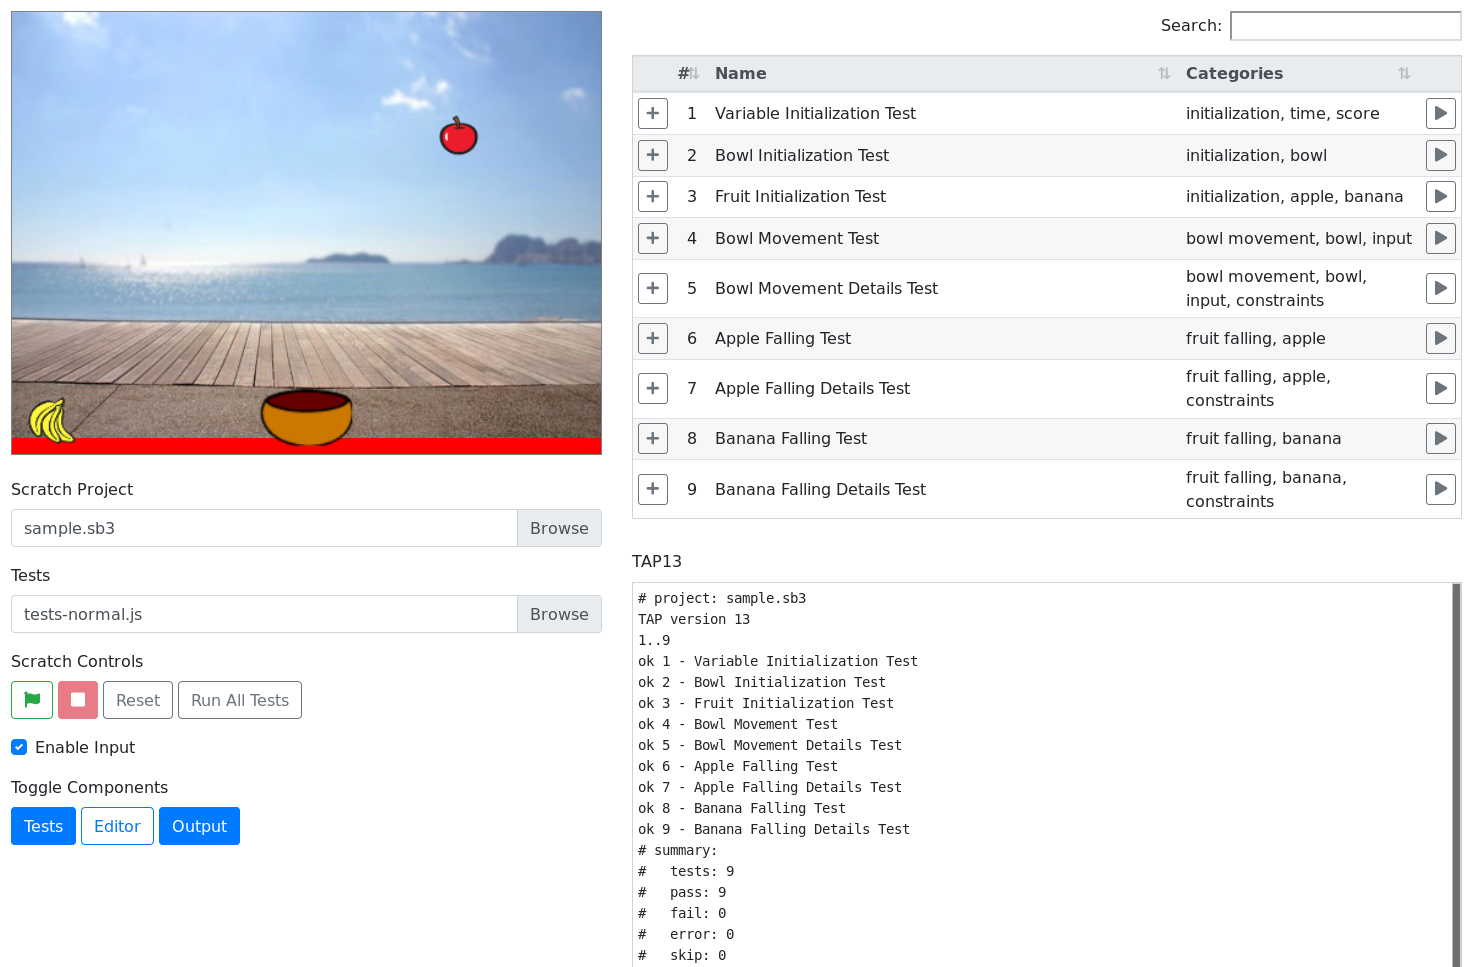
\includegraphics[width=0.85\textwidth]{whisker-gui}
    \caption{Screenshot of Whisker's web GUI}
    \label{fig:whisker_gui}
\end{figure}



% Therefore, we only concern ourselves with ...

% We are going to deal with this problem by creating a wrapper around Scratch,
% which can be used to simulate input and access information about the sprites which make up the output.
% Tests can then use methods, which the wrapper provides, instead of manually interacting with the Scratch program.

% Therefore, additional computations by the testing procedure must be fast enough to avoid interfering with the program under test.

\section{Public Interface}
\label{sec:public_interface}

% \begin{enumerate}[(1)]
%     \item Registered callbacks are executed.
%         This is done before anything else, so they can register (or unregister) inputs before the program is run.
%     \item Random inputs are chosen, randomized, and then registered as normal inputs.
%     \item Inputs, which are due, are performed.
%     \item Sprites' \texttt{old} values, which contain attributes from the last step, are updated.
%         This is done right before the Scratch program is stepped, so the program can change the sprites right after,
%         and no code has to deal with incorrect \texttt{old} values.
%     \item Scratch's step function is called to advance the program.
%     \item Callbacks, which are registered to run after the Scratch step, are executed.
%         With this, callbacks can unregister constraints after the program was stepped.
% \end{enumerate}

Automating Scratch allows us to write tests for Scratch in a unit-test-like fashion.
Whisker loads and starts the program before each test starts.
By doing this, every test starts with a fresh instance of the program in the exact same state.
% The test code can then interact with the program in order to produce a desired situation and check how the program behaves through assertions.
\parspace

Tests use a test driver object to automate Scratch through Whisker.
Whisker's own testing framework automatically passes the test driver object to its tests as an argument,
but tests written for other testing frameworks may have to acquire the test driver in their test code.
Whisker offers an interface to create and configure the test driver object for this purpose.
Listing~\ref{fig:examples_of_how_to_acquire_the_test_driver} shows code examples for both possibilities.
\parspace

\begin{listing}[htpb]
    \centering
    \begin{subfigure}[b]{.35\textwidth}
        \begin{minted}[autogobble, breaklines, linenos, fontsize=\scriptsize, framesep=2mm, frame=lines]{javascript}
            async function test (t) {
                ...
            }
        \end{minted}
        \vspace{-\bigskipamount}
        \caption{Getting the test driver passed as a parameter}
    \end{subfigure}
    \hspace{.05\textwidth}
    \begin{subfigure}[b]{.50\textwidth}
        \begin{minted}[autogobble, breaklines, linenos, fontsize=\scriptsize, framesep=2mm, frame=lines]{javascript}
            async function test () {
                const whisker = new WhiskerUtil(vm, project);
                whisker.prepare();
                const t = whisker.getTestDriver();
                whisker.start();
                ...
            }
        \end{minted}
        \vspace{-\bigskipamount}
        \caption{Manually acquiring the test driver through Whisker's interface}
    \end{subfigure}
    \caption{Examples of how to acquire the test driver}
    \label{fig:examples_of_how_to_acquire_the_test_driver}
\end{listing}

\mnote{TODO: rewrite this, better explanations and code examples\\TODO: properties depend on time $\rightarrow$ ''old'' values}
The following list will give an overview of Whisker's basic functions.
The test driver will be denoted as $t$ in example code snippets.

\begin{itemize}
    \item \textbf{Simulate Input.}
        \mnote{TODO: check if key is pressed}
        By simulating Scratch's main input methods, the test can control the tested program.
        The goal is to simulate a user interacting with the program.
        Therefore, this is the only way the test can manipulate the program.
        The possible input includes mouse movement, mouse button presses, keyboard key presses and entering answers to ask blocks.
        \begin{javascriptcode}
            t.addInput(1000, {
                device: 'keyboard',
                key: 'right arrow',
                isDown: true
            });
        \end{javascriptcode}
    \item \textbf{Access Information.}
        \mnote{Explain how in the implementation chapter (objects)}
        The testing utility can be used to access sprites and variables of the program.
        This makes it possible to gather information about anything, which is displayed on the stage.
        Analyzing Scratch's visual output would otherwise be very difficult.
        The provided sprite attributes include the sprite's position, rotation, size, current costume, speech bubble text, etc..
        The values of the program's variables can also be accessed.
        These variable values can usually be displayed to the user in Scratch's graphical output, and are commonly used in Scratch programs to convey information to the user.
        \begin{javascriptcode}
            const sprite = t.getSprite('Sprite1');
            const stage = t.getStage();
            const variable = stage.getVariable('my variable');
            console.log(sprite.x);
            console.log(variable.value);
        \end{javascriptcode}
    \item \textbf{Control the program execution.}
        The test is able to control when and for how long the program under test is run.
        In the beginning of the test, the program starts in a paused state with the green flag already pressed.
        The test can then run (resume) the program for a certain time, or until a condition is met.
        The green flag can also be pressed again in order to restart the program, which can, for example, be useful for testing programs, that use randomness.
        \begin{javascriptcode}
            await t.runForTime(1000);
            await t.runUntil(() => sprite.x > 100));
            t.greenFlag();
        \end{javascriptcode}
    \item \textbf{Register Callbacks.}
        The test can register callbacks, which get called every time Scratch renders a new picture.
        This allows the test to track the information, which the user would normally see, while the program is running.
        \begin{javascriptcode}
            const spritePositions = [];
            const callback = t.addCallback(() => spritePositions.push(sprite.pos));
            callback.disable();
            callback.enable();
        \end{javascriptcode}
    \item \textbf{Register constraints.}
        \mnote{''In the second and third case, it is up to the test code to check which constraints failed and react accordingly.''}
        By registering constraints, the test can define conditions that must always hold true.
        Constraints are done through special callbacks, which perform assertions.
        For example, this can be used to define that a certain sprite must always be visible.
        \begin{javascriptcode}
            const constraint = t.addConstraint(() => {
                t.assert.ok(sprite.visible === true)
            });
            constraint.disable();
            constraint.enable();
        \end{javascriptcode}
\end{itemize}

\noindent Despite being possible in theory, Whisker does not provide the means to execute single scripts or blocks of the program directly.
\mnote{TODO: really write about grading here?}
It only allows executing the program as a whole.
This has two reasons.
Since the main goal for this testing approach is automated grading, one test suite is possibly executed on a large number of different implementations.
Therefore, we don't want to concern ourselves with the internals of the program, since they may change from program to program.
Secondly, executing single scripts could also lead to unexpected behaviour in the program, because scripts in typical Scratch programs often depend on other scripts, which run in parallel.
% This is mainly due to the game-like nature of usual Scratch programs.
% They often feature multiple sprites running loops in order to be interactive.

\section{Challenges of this Approach}
\label{sec:appraoch_challenges}

% \begin{itemize}
%     \item This approach allows to test programs with most of Scratch's functionality.
%         Apart from sounds and extensions, anything, which Scratch has to offer, can be tested with this approach.
%         In contrast, ITCH's previous testing approach limited Scratch programs to textual IO.
%     \item Tests are easily understood, because they control the program like a normal person would.
%     \mnote{Can't state this without proof $\rightarrow$ "we believe" or similar}
%         This is important, because students, whose programs are supposed to be tested later,
%         could be allowed to run tests on their programs themselves during development.
%         This way, students could easily receive valuable feedback about the correctness of their implementations.
%         Therefore, it is beneficial to use tests, whose actions and purposes are easily understood by students.
% \end{itemize}

This section highlights various challenges that can make testing with this approach difficult.
\parspace

\textbf{General testing challenges.}
Firstly, automated testing in general introduces some challenges.
For one thing, programs have to be well specified, since testing relies on the program's specification.
Therefore, if the specification is too vague, testing can become difficult.
Tests for imprecise specifications potentially need to consider more possible cases of how the program could behave.
Likewise, conflicting interpretations of the specification between the test and the program may result in false negative test outcomes.
Also, since we only test the program as a whole, testing a single part of the program can be difficult.
If some feature of the program under test depends on another feature being implemented correctly,
but the latter does not work, the first feature can not be tested properly.
\parspace

\textbf{Addressing sprites and variables.}
In order to access information about sprites and variables, they need to be addressed in some way.
Sprites can be addressed by any of their attributes, for example by their position or by their name.
Nevertheless, if a sprite, that is needed for the test, can not be found, the test can not work properly.
This can be a problem if a Scratch program deviates from the specification or from a provided template.
However, errors like this can easily be detected through test reports.
% Probably the easiest way to handle this is to give students a Scratch project with the sprites and variables already in place
% as a template so the sprites and variables have the same name in each student solution.
\parspace

\textbf{Missing initialization.}
Another challenge are programs which are missing initialization and are saved in a bad state.
The Scratch GUI picks up where the last execution left off when the green flag is pressed.
Therefore, students might not initialize their program properly,
which can cause it to behave incorrectly sometimes when the green flag is pressed..
A program with missing initialization may be saved in a bad state,
meaning the program will behave incorrectly the next time it is started.
Since we restore the same state in the beginning of each test case,
such a program will always behave incorrectly during the tests although the implementation might be mostly correct.
\parspace

\textbf{Time-displaced events.}
Programs may have events that are supposed to trigger certain actions.
For example, a sprite touching another sprite may cause a variable to be incremented.
But the exact timing for the triggered action is often unknown, because the event is detected through a loop.
Therefore, tests have to check if the action happens in a time interval after the event occurred.
This may be done by tracking timestamps of the event and the action, and comparing these timestamps,
but this is expensive to do.
\parspace

\chapter{Using Constraints For Flexible Test Inputs}
\label{cha:using_constraints_for_flexible_test_inputs}

This section will describe why separating control of the program under test from the test code can be beneficial,
and how this can be achieved by defining constraint, that are checked in the background.

\section{Input-Independent / Constraint-only Tests}
\label{sec:input_independent_constraint_only_tests}

\mnote{TODO: ''constraint-only''}
Usually, tests will provide the program under test with inputs and check the resulting outputs.
However, in many cases, a different approach is possible as well.
Tests may use other sources of input and simply observe if the program's output is correct for the input provided by the source.
QuickCheck~\cite{quickcheck} by Claessen et al., for example, uses this principle, to test the correctness of Haskell programs.
In order to do so, tests define conditions, which the program must comply with.
QuickCheck then automatically generates input for the program and checks if the defined conditions hold.
\parspace

Scratch programs can often be tested in a similar way.
But in order to be able to do this, tests have to be made independent of the simulated input on the program.
This will not just enable us to test with generated input, but with other input sources as well.
For example, the program could be manually controlled by a person, or input could be recorded and played back.
Whisker also offers its own method of automated input generation by randomizing a set of inputs,
which are either provided by the test itself, or deduced by analyzing the program code (see section~\ref{sec:automated_input_generation} for more information on this).
\parspace

Scratch tests can often be made independent of inputs, and Whisker provides the means to do this.
Using constraints allows us to define conditions, which the program must hold.
Constraints check the program's compliance to the conditions by continually performing assertions throughout the program execution.
Since this is done entirely in the background while the program under test is running, we can define constraints and just let the program run for some time.
This way, it does not matter in what state the program is during its execution, or what inputs it is receiving.
If a condition does not hold, the respective constraint fails.

\section{Testing Procedure}
\label{sec:constraint_testing_procedure}

Figure~\ref{fig:input_independent_testing_procedure} shows a testing procedure, which uses the aforementioned approach to test independently of the simulated input.
We will go through each step of the procedure with the aid of an example.
Consider a program with a single sprite, which is supposed to move to the right precisely when the right arrow key is pressed.
We want to write a test to check if the sprite's movement works correctly.

\begin{figure}[htpb]
    \centering
    \tikzset{>=latex,
           arrow/.style={draw, -{Latex[length=1.5mm, width=1.5mm]}},
             box/.style={draw, text width=4.3cm, minimum height=0.7cm, text centered, rounded corners},
             num/.style={draw, circle, inner sep=0.6mm, text centered},
               h/.style={fill=blue!10}}

    \begin{tikzpicture}[scale=0.9, every node/.style={scale=0.9}]
        \node[box]    at (0.2, 5.75) (initialize)  {Give the program some time to Initialize};
        \node[box, h] at (0.2, 4.25) (tracking)    {Setup information tracking};
        \node[box, h] at (0.2, 3.0)  (constraints) {Register constraints};
        \node[box]    at (0.2, 2.0)  (inputs)      {(Simulate Inputs)};
        \node[box]    at (0.2, 1.0)  (run)         {Run the program};
        \node[box, h] at (0.2, 0.0)  (verify)      {Verify tested situation};

        \node[num] at (-2.6, 5.75) (one)   {1};
        \node[num] at (-2.6, 4.25) (two)   {2};
        \node[num] at (-2.6, 3.0)  (three) {3};
        \node[num] at (-2.6, 2.0)  (four)  {4};
        \node[num] at (-2.6, 1.0)  (five)  {5};
        \node[num] at (-2.6, 0.0)  (six)   {6};

        \draw[arrow]
               (0.2,  6.6)
            -- (initialize)
            -- (tracking)
            -- (constraints)
            -- (inputs)
            -- (run)
            -- (verify)
            -- (0.2, -0.8);
    \end{tikzpicture}

    \caption{Input-independent testing procedure}
    \label{fig:input_independent_testing_procedure}
\end{figure}

\begin{enumerate}
    \item[(1)] \textbf{Setup information tracking.}
        \mnote{TODO: Update for new example}
        The constraint, which we will have to define later, will depend on information, which is not always available.
        Because we need to determine the sprite's movement direction, we have to know the position of the sprite from the last rendered frame.
        In order to track this, we add a callback, which tracks the sprite's last position.
        (Note: Whisker makes the sprites' attributes from the last rendered frame available through \texttt{sprite.old}, but we are going to ignore this for the sake of the example)
        \begin{javascriptcode}
            let oldX;
            t.addCallback(() => {
                oldX = sprite.x;
            });
        \end{javascriptcode}
    \item[(2)] \textbf{Register constraints.}
        Now, that we know the sprite's last position, we can determine if, and in which direction, it has moved since the last frame.
        We check its movement dependent on what key is currently pressed.
        \begin{javascriptcode}
            t.addConstraint(() => {
                if (t.isKeyDown("right arrow")) {
                    t.assert.ok(sprite.x > oldX);
                } else {
                    t.assert.ok(sprite.x === oldX);
                }
            });
        \end{javascriptcode}
    \item[(3,4)] \textbf{Simulate Inputs, Run the program.}
        \setcounter{enumi}{4}
        Now we can register inputs if we want to, and then we can run the program.
        How we simulate inputs, or if we perform inputs manually, does not matter for the test, of course.
        \begin{javascriptcode}
            t.detectRandomInputs();
            await t.runForTime(5000);
        \end{javascriptcode}
    \item[(5)] \textbf{Verify tested situation.}
        If our source of input does not guarantee, that the right arrow key gets pressed at all, we risk the chance of a false positive test result,
        because then, part of our constraint does not ever get checked.
        In this case, we also want set up tracking for the key press in the beginning,
        and then skip the test if the key does not get pressed at all in the end.
        \begin{javascriptcode}
            let rightPressed = false;
            const detectRight = t.addCallback(() => {
                if (t.isKeyDown("right arrow")) {
                    rightPressed = true;
                    detectRight.disable();
                }
            });

            ...

            t.assume.ok(rightPressed);
        \end{javascriptcode}
\end{enumerate}

\begin{listing}[htpb]
    \centering
    \begin{subfigure}[b]{.35\textwidth}
        \centering
        \begin{minted}[autogobble, breaklines, linenos, fontsize=\tiny, framesep=2mm, frame=lines]{javascript}
            const sprite = t.getSprite('Sprite1');

            /* Give the program some time to initialize. */
            await t.runForTime(100);

            let oldX = sprite.x;

            await t.runForTime(1000);

            /* Sprite should not move when no key
               is pressed. */
            t.assert.ok(oldX === sprite.x);

            t.inputImmediate({
                device: 'keyboard',
                key: 'right arrow',
                isDown: true
            });

            await t.runForTime(1000);

            /* Sprite should move right when the
               right arrow key is pressed. */
            t.assert.ok(oldX < sprite.x);
        \end{minted}
        \caption{Normal test}
    \end{subfigure}
    \hspace{.08\textwidth}
    \begin{subfigure}[b]{.55\textwidth}
        \centering
        \begin{minted}[autogobble, breaklines, linenos, fontsize=\tiny, framesep=2mm, frame=lines]{javascript}
            let sprite = t.getSprite('Sprite1');

            /* (1) Give the program some time to initialize. */
            await t.runForTime(100);

            /* When the last right arrow key press started. */
            let startPressedTime, startReleasedTime;
            /* When the right arrow key was last recorded as pressed / released. */
            let pressedTime, releasedTime;
            /* When the sprite was last recorded as moving right / staying still. */
            let movedRightTime, stayedStillTime;
            /* If the right arrow key was pressed in the previous step. */
            let previouslyPressed = t.isKeyDown('right arrow');
            /* If the right arrow key was pressed at all. */
            let pressed = false, released = false;

            /* (2) Track when the right arrow key is being pressed,
             * and when it is released. */
            const trackArrowPressCb = t.addCallback(() => {
                const currentTime = t.getTotalTimeElapsed();
                if (t.isKeyDown('right arrow')) {
                    pressed = true;
                    pressedTime = currentTime;
                    if (!previouslyPressed) {
                        startPressedTime = currentTime;
                        previouslyPressed = true;
                    }
                } else {
                    pressed = false;
                    releasedTime = currentTime;
                    if (previouslyPressed) {
                        startReleasedTime = currentTime;
                        previouslyPressed = false;
                    }
                }
            });

            /* (2) Track when the sprite is moving to the right,
             * and when it is staying still. */
            const trackSpriteMoveCb = t.addCallback(() => {
                if (sprite.x > sprite.old.x) {
                    movedRightTime = t.getTotalTimeElapsed();
                } else if (sprite.x === sprite.old.x) {
                    stayedStillTime = t.getTotalTimeElapsed();
                }
            });

            /* (3) Check if the sprite only moves when the right arrow
             * key was pressed, and if it doesn't move when the key was
             * not pressed. */
            const spriteMoveConstraint = t.addConstraint(() => {
                const currentTime = t.getTotalTimeElapsed();
                if (currentTime > startPressedTime + 100) {
                    t.assert.ok(pressedTime - movedRightTime <= 100,
                                'Sprite must move right when right arrow key is pressed.');
                }
                if (currentTime > startReleasedTime + 100) {
                    t.assert.ok(releasedTime - stayedStillTime <= 100,
                                'Sprite must not move right when right arrow key is not pressed.');
                }
            });

            /* (4) Some code, which registers inputs. Or nothing if
             * inputs are done manually. For example, generated input: */
            t.setRandomInputInterval(250);
            t.detectRandomInputs();

            /* (5) Run the program. */
            await t.runForTime(5000);

            /* (6) Check if the right arrow key was pressed at all,
             * and if it was ever released. */
            t.assume.ok(pressedTime >= 0, 'Right arrow key must be pressed.');
            t.assume.ok(releasedTime >= 0, 'Right arrow key must be released.');
        \end{minted}
        \caption{Input-independent test}
        \label{fig:normal_input_independent_test_comparison_constraint}
    \end{subfigure}
    \caption{Comparison of normal tests and an input-independent tests}
    \label{fig:normal_input_independent_test_comparison}
\end{listing}
\parspace

Figure~\ref{fig:normal_input_independent_test_comparison} shows the resulting test code for the example
and compares it to a similar test, which simulates inputs deliberately to check the sprite's movement.
We can easily see, that this approach is quite a bit more costly than the more normal approach.
But at the same time, the input-independent testing procedure is able to scale better than the other testing procedure.
Once enough tracking is set up, writing constraints becomes easy and does not requires little code.
At the same time, because the constraints are isolated from the program execution itself,
many constraints can possibly be combined into a single test.
For this purpose, Whisker offers an option to disable failed constraints instead of failing the entire test.
Hence, the test can simply check which constraints failed at the end, and let Whisker generate a test report from them.

\section{Resetting the Program During a Test}
\label{sec:resetting_the_program_during_a_test}

For testing with randomly generated input, programs often need to be reset multiple times inside of one test execution,
because the test could get stuck in some state of the program.
To reset a Scratch program, we may simply press the green flag button again,
but we also need to consider the tracked information as well as the registered callbacks and constraints when resetting the program under test.
Figure~\ref{fig:resetting_the_program_under_test_procedure} shows a procedure that may be used to reset the program under test.
This procedure replaces step $4$ (Run the program) in the input-independent testing procedure (see Figure~\ref{fig:input_independent_testing_procedure}).
Additionally the code example in Listing~\ref{fig:resetting_the_program_under_test_example}
implements this procedure for the example in Listing~\ref{fig:normal_input_independent_test_comparison_constraint}.
\parspace

Sometimes, information may need to be tracked across resets in order to determine what events occurred in the program during the whole test execution.
This information may be needed to rule out constraints, whose situation never occurred, after the test execution.
An example for this are the variables \texttt{pressed} and \texttt{released} in Listing~\ref{fig:normal_input_independent_test_comparison_constraint}.

\begin{figure}[htpb]
    \centering
    \begin{subfigure}[m]{.3\textwidth}
        \centering
        \tikzset{>=latex,
               arrow/.style={draw, -{Latex[length=1.5mm, width=1.5mm]}},
                 box/.style={draw, text width=4.3cm, minimum height=0.7cm, text centered, rounded corners},
                 num/.style={draw, circle, inner sep=0.6mm, text centered},
                   h/.style={fill=blue!10}}

        \begin{tikzpicture}[scale=0.9, every node/.style={scale=0.9}]
            \node[box, h] at (0.2,  6.75) (suspendcb)  {Suspend Information Tracking};
            \node[box, h] at (0.2,  5.50) (suspendcn)  {Suspend Constraints};
            \node[box, h] at (0.2,  4.25) (resetinfo)  {Reset per-run information};
            \node[box]    at (0.2,  2.25) (greenflag)  {Press the green flag and give the program some time to Initialize};
            \node[box]    at (0.2,  0.75) (spriteref)  {Get new sprites};
            \node[box, h] at (0.2, -0.75) (activatecb) {Activate Information Tracking};
            \node[box, h] at (0.2, -2.00) (activatecn) {Activate Constraints};
            \node[box]    at (0.2, -3.00) (run)        {Run the program};


            \node[num] at (-2.6,  6.75) (one)   {1};
            \node[num] at (-2.6,  5.50) (two)   {2};
            \node[num] at (-2.6,  4.25) (three) {3};
            \node[num] at (-2.6,  2.25) (four)  {4};
            \node[num] at (-2.6,  0.75) (five)  {5};
            \node[num] at (-2.6, -0.75) (six)   {6};
            \node[num] at (-2.6, -2.00) (seven) {7};
            \node[num] at (-2.6, -3.00) (eight) {8};

            \draw[arrow]
                   ( 0.2,  7.6)
                -- (suspendcb)
                -- (suspendcn)
                -- (resetinfo)
                -- (greenflag)
                -- (spriteref)
                -- (activatecb)
                -- (activatecn)
                -- (run)
                -- ( 0.2, -3.8);

            % \draw[-, rounded corners]
            %        ( 0.2, -2.8)
            %     -- (-3.4, -2.8)
            %     -- (-3.4,  7.7)
            %     -- ( 0.2,  7.7);
        \end{tikzpicture}
        \caption{Procedure for resetting the program under test}
        \label{fig:resetting_the_program_under_test_procedure}
    \end{subfigure}%
    \hspace{.13\textwidth}%
    \begin{subfigure}[m]{.55\textwidth}
        \centering
        \begin{minted}[autogobble, breaklines, linenos, fontsize=\scriptsize, framesep=2mm, frame=lines]{javascript}
            for (let i = 0; i < 10; i++) {
                /* (1) Suspend information tracking. */
                trackArrowPressCb.disable();
                trackSpriteMoveCb.disable();

                /* (2) Suspend constraints. */
                spriteMoveConstraint.disable();

                /* (3) Reset per-run information
                   (keep values of 'pressed' and 'released'). */
                spriteMoveConstraint.disable();
                startPressedTime = startReleasedTime = undefined;
                pressedTime = releasedTime = undefined;
                movedRightTime = stayedStillTime = undefined;
                previouslyPressed = t.isKeyDown('right arrow');

                /* (4) Press the green flag and give the program
                   some time to Initialize. */
                t.greenFlag();
                await t.runForTime(100);

                /* (5) Get new sprites. */
                let sprite = t.getSprite('Sprite1');

                /* (6) Activate information tracking. */
                trackArrowPressCb.enable();
                trackSpriteMoveCb.enable();

                /* (7) Activate constraints. */
                spriteMoveConstraint.enable();

                /* (8) Run the program. */
                await t.runForTime(5000);
            }
        \end{minted}
        \vspace{-\bigskipamount}
        \caption{Example code for resetting the program under test (extends Listing~\ref{fig:normal_input_independent_test_comparison_constraint})}
        \label{fig:resetting_the_program_under_test_example}
    \end{subfigure}

    \caption{Resetting the program under test}
    \label{fig:resetting_the_program_under_test}
\end{figure}


% Register Callbacks for Information Tracking (per run for constraints and across runs to rule out constraints in the end)
% Register Constraints
%
% repeat:
%     Suspend Information Tracking Callbacks
%     Suspend Constraints
%
%     Reset Per Run Information
%
%     Press Green Flag
%     Run the Program For Short Time to Initialize It
%
%     Activate Information Tracking Callbacks
%     Activate Constraints
%
%     Run the Program
%
% Check Across-Run Information to Disable Constraints, whose situation to check did not occur
% Generate test report


% \begin{figure}[htpb]
%     \centering
%     \begin{subfigure}[b]{.45\textwidth}
%         \centering
%         \tikzset{>=latex,
%                  box/.style={draw, text width=4.3cm, minimum height=0.7cm, text centered, rounded corners},
%                  num/.style={draw, circle, inner sep=0.6mm, text centered},
%                    h/.style={fill=blue!10}}
%
%         \begin{tikzpicture}
%             \node[box] at ( 0.2,  3.0) (run)        {Run the program};
%             \node[box] at ( 0.2,  2.0) (inputs)     {Simulate inputs};
%             \node[box] at ( 0.2,  1.0) (checks)     {Perform checks};
%
%             \node[num] at (-2.6,  3.0) (one)   {1};
%             \node[num] at (-2.6,  2.0) (two)   {2};
%             \node[num] at (-2.6,  1.0) (three) {3};
%
%             \draw[->]
%                    ( 0.2,  4.8)
%                 -- (run)
%                 -- (inputs)
%                 -- (checks)
%                 -- ( 0.2, -1.0);
%
%             \draw[shorten >= 2pt, rounded corners, dashed, ->]
%                    ( 0.2,  0.0)
%                 -- (-3.4,  0.0)
%                 -- (-3.4,  4.0)
%                 -- ( 0.2,  4.0);
%         \end{tikzpicture}
%
%         \caption{Normal Test Procedure}
%         \label{fig:normal_test_procedure}
%     \end{subfigure}
%     \begin{subfigure}[b]{.45\textwidth}
%         \centering
%         \tikzset{>=latex,
%                  box/.style={draw, text width=4.3cm, minimum height=0.7cm, text centered, rounded corners},
%                  num/.style={draw, circle, inner sep=0.6mm, text centered},
%                    h/.style={fill=blue!10}}
%
%         \begin{tikzpicture}
%             \node[box] at ( 0.2,  4.25) (tracking)    {Setup tracking of information};
%             \node[box] at ( 0.2,  3.0)  (constraints) {Register constraints};
%             \node[box] at ( 0.2,  2.0)  (run)         {Run the program};
%             \node[box] at ( 0.2,  1.0)  (inputs)      {(Simulate Inputs)};
%             \node[box] at ( 0.2,  0.0)  (filter)      {Filter constraints};
%
%             \node[num] at (-2.6,  4.25) (one)   {1};
%             \node[num] at (-2.6,  3.0)  (two)   {2};
%             \node[num] at (-2.6,  2.0)  (three) {3};
%             \node[num] at (-2.6,  1.0)  (four)  {4};
%             \node[num] at (-2.6,  0.0)  (five)  {5};
%
%             \draw[->]
%                    (tracking)
%                 -- (constraints)
%                 -- (run)
%                 -- (inputs)
%                 -- (filter)
%                 -- ( 0.2, -1.0);
%         \end{tikzpicture}
%
%         \caption{Constraint-only Test Procedure}
%         \label{fig:constraint_only_test_procedure}
%     \end{subfigure}
%     \caption{Comparison of the procedure of normal tests and constraint-only tests}
%     \label{fig:comparison_of_the_procedure_of_normal_tests_and_constraint_only_tests}
% \end{figure}
